
\documentclass[manuscript]{aastex}
\newcommand{\myemail}{gbrunner@rice.edu}

\shorttitle{Mapping Molecular Hydrogen in NGC 5194}
\shortauthors{Brunner et al.}


\begin{document}

\title{Mapping $\mathrm{H_2}$ Excitation and Mass across NGC 5194 with the Spitzer IRS}

\author{Gregory Brunner\altaffilmark{1,2}}
\affil{Department of Physics and Astronomy, Rice University, \\
    Houston, TX 77005}
\email{gbrunner@ipac.caltech.edu, gbrunner@rice.edu}

\author{Kartik Sheth\altaffilmark{3}, Lee Armus\altaffilmark{3}, and George Helou\altaffilmark{3}}
\affil{Spitzer Science Center, Pasadena, CA 91125}

\author{Eva Schinnerer\altaffilmark{4}}
\affil{Max-Planck-Intit\"{u}t f\"{u}r Astronomie, Heidelberg, Germany}

\and 

\author{Stuart Vogel\altaffilmark{5} and Mark Wolfire\altaffilmark{5}}
\affil{Department of Astronomy, University of Maryland, College Park, MD 20741}

\altaffiltext{1}{Department of Physics and Astronomy, Rice University, Houston, TX 77005}
\altaffiltext{2}{Visiting Graduate Student Fellow, Spitzer Science Center, Caltech, Pasadena, CA}
\altaffiltext{3}{Spitzer Science Center, Caltech, Pasadena, CA}
\altaffiltext{4}{Max-Planck-Instit\"{u}t f\"{u}r Astronomie, Heidelberg, Germany}
\altaffiltext{5}{Department of Astronomy, University of Maryland, College Park, MD}


\begin{abstract}

We have mapped $\mathrm{H_2}$ pure rotational line emission for the $\mathrm{H_2}$ S(0), $\mathrm{H_2}$ S(1), $\mathrm{H_2}$ S(2), $\mathrm{H_2}$ S(3), $\mathrm{H_2}$ S(4), and $\mathrm{H_2}$ S(5) lines over a strip across NGC 5194 using the $Spitzer$ $Space$ $Telescope$ Infrared Spectrograph low resolution modules.  The $\mathrm{H_2}$ line intensity maps reveal differences in the molecular gas morphology of NGC 5194.  We use the $\mathrm{H_2}$ maps to examine the $\mathrm{H_2}$ excitation-temperature and mass across the galaxy.  We find that within our beam, $\mathrm{H_2}$ exists in a continuous distribution of temperatures across the galaxy.  We measure the $\mathrm{H_2}$ excitation-temperature of both the "warm" (T = 100 - 300 K) and "hot" (T = 400 - 1200 K) mass distributions traced by the  $\mathrm{H_2}$ S(0) - $\mathrm{H_2}$ S(2) and $\mathrm{H_2}$ S(2) - $\mathrm{H_2}$ S(5) lines, respectively.  We investigate the origin of the $\mathrm{H_2}$ emission by comparing the location of $\mathrm{H_2}$ emission and mass to photodissociation regions (traced by CO), shock-excited [O IV](25.89 $\micron$) emission, and X-ray dissociation regions from $Chandra$ observations.  We find that within the spiral arms, the $\mathrm{H_2}$ mass correlates with the CO (J = 1 - 0) emission; although, we see offsets in the location of the peaks in $\mathrm{H_2}$ mass and CO intensity.  Comparing $\mathrm{H_2}$ line intensity to CO intensity reveals that within the spiral arms, pure rotational $\mathrm{H_2}$ line emission is generally cospatial with CO emission indicating that the pure rotational $\mathrm{H_2}$ line emission is originating from the surface layers of dense molecular clouds associated with star-forming regions.  Within the  nuclear regions of NGC 5194, the hot $\mathrm{H_2}$ phase is copsatial with [O IV](25.89 $\micron$) emission and X-ray emission while the warm $\mathrm{H_2}$ is not.  Comparison between the X-ray emission and $\mathrm{H_2}$ line emission reveal that the $\mathrm{H_2}$ morphology is correlated with the X-ray morphology.

\end{abstract}

\keywords{galaxies: ISM --- galaxies: $\mathrm{H_2}$ --- galaxies: individual(NGC 5194)}

\section{Introduction}

Star formation and galactic evolution are inherently connected with molecular hydrogen ($\mathrm{H_2}$) within a galaxy.  In the Milky Way, all star formation occurs in molecular clouds (Blitz 1995); although, not all molecular clouds are actively forming stars.  In galaxies, star formation is triggered whenever the molecular gas surface density is enhanced, for example, by a spiral density wave (Vogel et al. 1988), by increased pressure as in galactic nuclei (Young and Devereux 1991),  due to the hydrodynamic shock along the leading edge of bars, and in the transition region at the ends of bars (Sheth et al. 2000, Kenney and Lord 1991).  Although the connection between star formation and molecular gas is well-established, the exact mechanisms for initiating, controlling, and inhibiting star formation are not well-known.

%Much of our knowledge of the conditions of the molecular gas in galaxies came from studies of CO emission and rotational-vibrational transitions of $\mathrm{H_2}$ in the near-infrared.  CO rotational line emission directly traces the mass of the coldest (T = 5 - 100 K) $\mathrm{H_2}$ while the near-infrared  $\mathrm{H_2}$ emission traces the hot (T  $\geq$ 1000 K) $\mathrm{H_2}$.  The CO (J = 1 - 0) line at 2.6 mm has served as a means to infer the mass of the coldest (T = 5 - 10 K) $\mathrm{H_2}$, which, owing to a lack of a permanent dipole moment, is undetectable in cold molecular clouds.  Studies of the near-infrared rovibrational emission have been hindered due to the low surface brightness of the rovibrational lines in galaxies (citation).  Though the $\mathrm{H_2}$ 2-1 S(0) line has been mapped across several galaxies (citation), there have been very few studies of the near-infrared rovibrational $\mathrm{H_2}$.

The Whirlpool Galaxy (M51a, NGC 5194) is a nearby, face-on galaxy that has been extensively studied in X-rays (Palumbo et al. 1985,  Terashima et al. 2001); UV, optical (Scoville et al. 2001), and IR (Calzetti et al. 2005); submillimeter (Matsushita et a. 2004); millimeter (Helfer and Blitz 1997); and radio wavelengths (Murphy et al. 2005).   At a distance of 9.6 Mpc (Sandage and Tammann, 1975), its proximity, orientation, and morphology make it an ideal target for studies of the interstellar medium (ISM) across distinct dynamical, chemical, and physical environments in a galaxy.  Studies have revealed variations in CO emission and UV radiation field, metallicity gradients, and temperature across the galaxy.  Thus, it has been called a $Rosetta$ $Stone$ for galaxy evolution (Scoville and Young, 1983).  

The Spitzer Space Telescope Infrared Spectrograph (IRS) (Houck et al. 2004) is a powerful tool for observing the $\mathrm{H_2}$  within galaxies and thus deciphering the evolution of M51a.  The Spitzer IRS low resolution modules cover 5 - 38 $\micron$ (SL, 5 - 14 \micron; LL, 14 - 38 \micron) giving observers access to the lowest pure rotational lines of $\mathrm{H_2}$. These lines trace the warm (T = 100 - 1000K) molecular gas and are important diagnostics of the ISM allowing for the determination of the $\mathrm{H_2}$ excitation-temperature, mass, and ortho-to-para ratio of $\mathrm{H_2}$.  Thus, by understanding the pure rotational $\mathrm{H_2}$ line emission from a galaxy, constraints can be placed on the energy injection mechanisms (i.e. radiative heating, shocks, turbulence) that heat the molecular gas phases in the ISM.

In this paper, we present spatially resolved observations of the $\mathrm{H_2}$ rotational lines across a radial strip of NGC 5194.  Using the Spitzer IRS, we have spectrally mapped a radial strip (295" x 51" in the long low module and 324" x 57" in the short low module) across \object{NGC 5194} in order to understand the conditions of the warm (T = 100 -1000 K) molecular ISM across dynamically distinct environments.  From the spatially resolved IRS low resolution spectra, maps of emission from the six lowest pure rotational transitions of $\mathrm{H_2}$, the $\mathrm{H_2}$(0-0)S(0) (28.22 $\micron$), $\mathrm{H_2}$(0-0)S(1) (17.04 $\micron$), $\mathrm{H_2}$(0-0)S(2) (12.28 $\micron$), $\mathrm{H_2}$(0-0)S(3) (9.66 $\micron$), $\mathrm{H_2}$(0-0)S(4) (8.02 $\micron$), and $\mathrm{H_2}$(0-0)S(5) (6.91 $\micron$) lines were created.  These maps represent measurements of extinction corrected line flux across \objectname{NGC 5194} (presented in \S3.1).  Maps are used to determine the spatial distribution of the $\mathrm{H_2}$ excitation-temperature and mass across the galaxy(\S3.2).  The dominant excitation mechanism of $\mathrm{H_2}$ (photodissociation by UV photons, shocks, and/or x-ray dissociation) is determined in various regions across the galaxy by comparing the $\mathrm{H_2}$ distribution to CO (J = 1 - 0) emission (\S4.2), [OIV](25.89 \micron) emission (\S4.3), and x-ray emission (\S4.4).   

\section{Observations and Data Reduction}

\subsection{Spectral Data}

Spectra were obtained for \objectname{NGC 5194} using the two low-resolution modules of the Infrared Spectrograph in spectral mapping mode. In spectral mapping mode, we moved the IRS in a series of discrete steps settling at each position before beginning integration.  Half slit spacing were used for all integrations. Integration times in the SL and LL were 14.6 s.  Each slit position was covered twice.  In total, 1,412 spectra were taken in the SL while 100 were taken in the LL (including background observations).  SL integrations were taken perpendicular to the LL integrations in accordance with the SINGS radial strip mapping strategy specified in by Kennicutt et al. (2003).  Further details on the observation strategy are available on SST's Leopard for project ID 200138 (PI: K. Sheth).  Dedicated off source background observations were taken for the SL observations.  Backgrounds for the LL observations were taken from outrigger data collected while the spacecraft was mapping in the adjacent module. 

The spectra were assembled from the basic calibration data into spectral cubes for each module using CUBISM (Smith et al. 2007, in preparation).  CUBISM allows for the assembly of cubes, extraction of spectra, and creation of spectral maps.  Background subtraction and bad pixel removal was done within CUBISM.  The individual IRS spectra were processed using version S14.0 of the Spitzer Science Center pipeline.

In CUBISM, the SL and LL data cubes have resolutions of 1.85"/pixel and 5.08"/pixel.  The spatial resolution of the data cubes varies as a function of wavelength due to a wavelength dependent point spread function (PSF).  Though the pixels are square, the PSF is circular and expands in radius with increasing wavelength.  Thus, we define the spatial resolution at a given wavelength in the SL and LL data cubes as 
\begin{equation}
R_{SL}(\lambda) = 1".85 * \lambda/5.2 \micron
\end{equation}
and
\begin{equation}
R_{LL}(\lambda) = 5".08 * \lambda/14.0 \micron,
\end{equation}
respectively, where $\lambda$ is the wavelength.

Spectral maps of the $\mathrm{H_2}$S(0) - $\mathrm{H_2}$S(5) lines were created with PAHFIT (Smith et al. 2007), a robust mid-infrared spectral fitting routine.  PAHFIT decomposes an IRS low resolution spectrum allowing the recovery of the full flux of blended features.  This allows the recovery of the full line flux of the $\mathrm{H_2}$ features, including severely blended lines such as $\mathrm{H_2}$S(1), blended with the 17 $\micron$ PAH complex (Smith et al. 2004); $\mathrm{H_2}$S(2), blended with [NeII](12.8 $\micron$); and $\mathrm{H_2}$S(5), blended into [ArII](6.9 $\micron$). 

In order to run PAHFIT though the SL and LL data cubes, the grid of the SL1 data cube was interpolated to the grid of the SL2 data cube.  The data cubes were then concatenated into one SL cube.  The same procedure was used to concatenate the LL1 and LL2 data cubes into one LL data cube.  In regions where the first order (SL1, LL1) spectra overlapped with the second order (SL2, LL2) spectra, the first order spectra were scaled up to the second order spectra.  The concatenated data cubes were then smoothed spatially by a 3 x 3 pixel box to increase the signal to noise ratio of spectra.  Grouping spectra was also done to avoid pixel aliasing, which has the affect of creating a saw-tooth pattern in the continuum (CUBISM User Manual).  PAHFIT was then run through both the SL and LL data cubes.  The SL data cube was fit separately from the LL data cube.

PAHFIT decomposes every spectrum in both the SL and LL data cubes.  In doing so, PAHFIT returns fit parameters to the specified features in the spectrum.  These parameters include extinction-corrected integrated line flux, line FWHM, line equivalent width, and uncertainty.  The integrated flux measurements are extinction corrected within PAHFIT (see Smith et al. 2007 for the extinction curve).   While running PAHFIT through the data cubes, information concerning the position of each spectrum was retained.  This allows for the reconstruction of spectral feature (PAH, $\mathrm{H_2}$, ionization line) maps from the results of PAHFIT.  When using PAHFIT on an entire data cube, maps of every feature specified by PAHFIT were returned.  Additionally, the fit to each spectrum was retained and the fit to the continuum was reconstructed from internal PAHFIT functions.  From these two data cubes, a residual data cube and a continuum subtracted data cube were created for both the SL and LL data cubes.  These data cubes are crucial in determining the consistency of the fitted spectra.  In order to check the accuracy of the map of $\mathrm{H_2}$S(3) integrated flux, it was compared it to the image created from the continuum subtraction to the SL data cube. 

In using PAHFIT, the default values for the temperatures of the starlight and eight thermal dust continuum components were used to fit the continuum.  Additionally, the optical depth of the dust extinction at 9.7 $\micron$ and 18 $\micron$  were also fit.  This was especially important in recovering an accurate measurement of the $\mathrm{H_2}$S(3) 9.6 $\micron$ line in the 9.7 $\micron$ silicate absorption trough.

\subsection{CO Map}

The BIMA (Berkely Illinois Maryland Array) CO (J=1-0) map was acquired as a part of the BIMA Survey of  Nearby Galaxies (SONG) (Regan et al. 2001; Helfer et al. 2003). The CO map was mosaicked from 26 fields.  The beam size is 5.8 x 5.1 $\mathrm{arcsec}$ (220 x 190 $\mathrm{pc}$), the velocity channel width is 10 km $\mathrm{s^{-1}}$, and the root-mean-square (rms) noise level is 61 mJy $\mathrm{beam^{-1}}$.   

\subsection{X-ray Emission}

The map of x-ray emission from M51 was observed by the Advanced CCD Imaging Spectrometer (ACIS) on the $Chandra$ $X-Ray$ $Observatory$ on 20 June 2000.  The total integration time was 14,865 seconds.  Further details of the observations are presented in Terashima and Wilson (2001).

\section{Results}

\subsection{$\mathrm{H_2}$ Emission Maps}

Molecular Hydrogen emission has been detected across \objectname{NGC 5194}.  The $\mathrm{H_2}$ S(0), $\mathrm{H_2}$ S(1), $\mathrm{H_2}$ S(2), $\mathrm{H_2}$ S(3), $\mathrm{H_2}$ S(4), and $\mathrm{H_2}$ S(5) lines have been mapped across the radial  strip.  In figures 1 and 2, maps of the extinction corrected flux of the $\mathrm{H_2}$ S(0) - $\mathrm{H_2}$ S(5) lines are presented.  The $\mathrm{H_2}$S(0) and $\mathrm{H_2}$S(1) lines (figure 1) lie in the LL module of the IRS and the resolution of the maps are 10".2 and 6".17, respectively.  The $\mathrm{H_2}$ S(2), $\mathrm{H_2}$ S(3), $\mathrm{H_2}$ S(4), and $\mathrm{H_2}$ S(5) lines (figure 2) lie in the SL module of the IRS and these maps have spatial resolutions of 4".37, 3'.44, 2".85, and 2".46, respectively.  The differences in resolution between the $\mathrm{H_2}$ maps explains the relative smoothness of $\mathrm{H_2}$S(0) and $\mathrm{H_2}$S(1) maps compared to the $\mathrm{H_2}$S(2) - $\mathrm{H_2}$S(5) maps.  Table 2 lists the resolution of the maps.  The boxes around the maps represent the regions over which the lines were mapped.  

Maps reveal remarkable differences in the morphology of \objectname{NGC 5194}.  $\mathrm{H_2}$S(0) emission is strongest in the NW spiral arm with much lower levels of emission coming from the nucleus.  The $\mathrm{H_2}$S(1) emission peaks in the nucleus of the galaxy with strong emission in the NW and SE spiral arms.  In the $\mathrm{H_2}$S(0) and $\mathrm{H_2}$S(1) emission, we are able to resolve molecular hydrogen emission in the outer spiral arms at several kiloparsecs from the center of the galaxy.  While we have resolved molecular hydrogen emission in the outer spiral arms, the peaks in $\mathrm{H_2}$S(0) and $\mathrm{H_2}$S(1) emission within the arms do not align.

The higher resolution $\mathrm{H_2}$S(2) - $\mathrm{H_2}$S(5) maps also show different morphology to \objectname{NGC 5194}.  The $\mathrm{H_2}$S(2) map shows the strongest emission in the nuclear region of \objectname{NGC 5194}.  The $\mathrm{H_2}$S(3) line exhibits similar strong emission in the nuclear region; however, there appears to be a bar structure across the nucleus of the galaxy going north-to-south.  Again, we see offsets in the peak emission within the spiral arms of \objectname{NGC 5194}.  These offsets are real and indicate variations in the excitation-temperature in each region.

Maps of the $\mathrm{H_2}$S(4) and $\mathrm{H_2}$S(5) lines show a remarkably different morphology to the nuclear region of \objectname{NGC 5194}.  The $\mathrm{H_2}$S(5) nuclear emission follows the nuclear emission of the $\mathrm{H_2}$S(3) line, while the $\mathrm{H_2}$S(4) nuclear emission mirrors the $\mathrm{H_2}$S(2) emission.  This indicates variations in the excitation-temperature (further explored in section \S3.3).

Due to the sensitivity of the IRS low resolution module, we were unable to resolve $\mathrm{H_2}$S(4) and $\mathrm{H_2}$S(5) emission beyond the central region of \objectname{NGC 5194}.   For the same reason, we were unable to create maps of the $\mathrm{H_2}$S(6) (at 6.11 \micron) and $\mathrm{H_2}$S(7) (at 5.51 \micron) lines.  Deeper observations could reveal more complete maps of the $\mathrm{H_2}$S(4) and $\mathrm{H_2}$S(5) emission in \objectname{NGC 5194} in addition to allowing us to map the $\mathrm{H_2}$S(6) and $\mathrm{H_2}$S(7) lines across \objectname{NGC 5194}.

\section{Discussion}

\subsection{$\mathrm{H_2}$ Excitation-Temperature and Mass across NGC 5194}

The pure rotational lines of molecular hydrogen provide a powerful probe of the conditions of the ISM and place constraints on the energy injection processes that excite $\mathrm{H_2}$.  Knowledge of the extinction corrected flux of the $\mathrm{H_2}$S(0) - $\mathrm{H_2}$S(5) lines allow for the mapping of the excitation-temperature and number density (and consequently mass).  The excitation-temperature and mass can be modeled across the galaxy by creating excitation diagrams at every position across the strip of NGC 5194.  

Excitation diagrams across NGC 5194 were created from the maps of $\mathrm{H_2}$ emission.  Each map was smoothed and interpolated to the resolution of the $\mathrm{H_2}$ S(0) line.  The non-rectangular shape to the excitation-temperature and mass are due to the offset in alignment between the LL and SL strips.  Excitation diagrams across the strip were derived from the Boltzman equation in similar form to the Rigopoulou et al. (2002).
\begin{equation}
N_i/N = (g(i)/Z(\mathrm{T_{ex}}))exp(-T_i/\mathrm{T_{ex}})
\end{equation}
where $g(i)$ is the statistical weight of state $i$, Z($\mathrm{T_{ex}}$) is the partition function, $\mathrm{T_i}$ is the energy level of a given state, and $\mathrm{T_{ex}}$ is the excitation temperature.  N and $\mathrm{N_i}$ are the total column density and the column density of a given state $i$ and is determined directly from the measured extinction corrected flux by
\begin{equation}
N_i = flux(i)/(A(i)h\nu (i))
\end{equation}
where A($i$) and $\nu$($i$) are the A-coefficient and frequency of state $i$ and $h$ is Planck's constant.  Table 1 lists the values for the wavelength ($\lambda$($i$)), rotational state (J), A($i$), $\mathrm{T_i}$, and $g(i)$ of the pure rotational levels of $\mathrm{H_2}$ that lie in the wavelength range covered by the IRS low resolution modules. 

The excitation diagrams exhibit an ortho-to-para ratio (OPR) in the nuclear region 3 (in agreement with the value of the OPR of the nuclear region determined by SINGS (Roussel et al. 2007, in press); this is determined from the fit to the best two-component fit to the $\mathrm{H_2}$S(0) - $\mathrm{H_2}$ S(5) lines.  Outside of the nuclear region, poor detection of the $\mathrm{H_2}$ S(4) and $\mathrm{H_2}$ S(5) lines prevents the mapping of OPR across the disk; however, the lower J lines exhibit an OPR of 3 within the spiral arms.

In the nuclear region of \objectname{NGC 5194}, the excitation diagram is smooth and its slope decreases at higher rotational levels (Figure 3).  This indicates that there is a range of temperatures being sampled within the beam.  Similar behavior has been observed in extragalactic targets by surveys of Seyferts (Rigopoulou et al. 2002) and ULIRGS (Higdon et al. 2006).  The temperature of the �warm� (T = 100 - 300 K) $\mathrm{H_2}$ and the temperature of the �hot� (T = 400 - 1200 K) $\mathrm{H_2}$ can be determined from the excitation diagrams by fitting the $\mathrm{H_2}$S(0) - $\mathrm{H_2}$S(2) lines and the $\mathrm{H_2}$S(2) - $\mathrm{H_2}$S(5) lines respectively (as opposed to fitting all of the observed $\mathrm{H_2}$ rotational lines in order to derive a temperature of the warm $\mathrm{H_2}$).  

From a two-component fit to the excitation diagram, the excitation-temperature of the ``warm'' and ``hot'' components of $\mathrm{H_2}$, the ``warm'' and ``hot'' $\mathrm{H_2}$ mass have been mapped across \objectname{NGC 5194} (figures 4, 5, and 6).  In measuring the mass in $\mathrm{H_2}$, we determine the mass from the number density by multiplying the column density by the physical area within the beam (Rigopoulou et al. 2002).  At 9.6 Mpc (Sandage and Tammann 1975), 5.08 arcsec corresponds to 236.43 parsecs.  The maps of the mass distribution are in units of solar masses within a 55.899 $\mathrm{kpc^2}$ region.  

%is that right?

Figure 4 compares the warm $\mathrm{H_2}$ mass to the temperature distribution of the mass.  The gas is warmest in the central region of \objectname{NGC 5194} with the temperature ranging from 225K - 275 K in the center of the galaxy.  The gas is coolest within the spiral arms of \objectname{NGC 5194}.  The outer NW and SE spiral arms (at about 6-7 kpc from the center of the galaxy each) contain on the order of 10,000 $\mathrm{M_\sun}$ (within a 55.9 $\mathrm{kpc^2}$ region) and 6,000 $\mathrm{M_\sun}$ (within a 55.9 $\mathrm{kpc^2}$ region) of $\mathrm{H_2}$ (in the NW and SE arms, respectively) and the gas within the outer spiral arms ranges from 150 K at the center of the arms to about 225 K near the edges.  Within the central oooo $\mathrm{pc^2}$ of the galaxy, there is oooo $\mathrm{M_\sun}$ of warm $\mathrm{H_2}$ and oooooo $\mathrm{M_\sun}$ hot $\mathrm{H_2}$.  These values are consistent with the masses of $\mathrm{H_2}$ found in the central regions of Seyferts (Rigopoulou et al. 2002).  In NGC 5194, the IRS is sensitive to 375 $\mathrm{M_\sun}$ warm $\mathrm{H_2}$ and 5 $\mathrm{M_\sun}$ hot $\mathrm{H_2}$ within the beam (though the sensitivity to the hot $\mathrm{H_2}$ could be underestimated due to smoothing the $\mathrm{H_2}$S(2), $\mathrm{H_2}$S(3), $\mathrm{H_2}$S(4), and $\mathrm{H_2}$S(5) lines by a factor of ~ 3 times their resolution).

%enter values there

 Note that due to zero detection of $\mathrm{H_2}$ in some of the inner arm regions, we are unable to determine the temperature distribution across the entire strip.  This is evident towards the NW and SE edges of the radial strip.

The temperature and mass distribution of the hot $\mathrm{H_2}$ reveals a different picture (Figure 5).  There is significantly less mass in the hot $\mathrm{H_2}$ phase, on the order several hundred $\mathrm{M_\sun}$, depending on the region. The greatest amount of hot $\mathrm{H_2}$ is found within the nuclear region of \objectname{NGC 5194}; this is much different from the warm $\mathrm{H_2}$ that dominates the spiral arms.  The hot gas exhibits cooler temperatures within the central regions of \objectname{NGC 5194} and the spiral arms.  Temperatures are greater in the inter-arm regions where there is less $\mathrm{H_2}$.  

Due to the weakness of the $\mathrm{H_2}$S(2), $\mathrm{H_2}$S(3), $\mathrm{H_2}$S(4), and $\mathrm{H_2}$S(5) features beyond the spiral arms, the hot $\mathrm{H_2}$ excitation temperature and mass can not be mapped over the whole strip.  While the radial strip across \objectname{NGC 5194} is helpful is understanding the $\mathrm{H_2}$ excitation-temperature and mass across the disk of the galaxy, complete IRS low resolution coverage of \objectname{NGC 5194} with longer integration time is necessary in order to understand hot $\mathrm{H_2}$ distribution and the $\mathrm{H_2}$ OPR across the whole galaxy.

%\subsection{Radial Variations in the Warm and Hot $\mathrm{H_2}$ Excitation-Temperature and Mass}

\subsection{Distinguishing the $\mathrm{H_2}$ Excitation Mechanisms}

Previous studies of pure rotational H2 emission in galaxies have used aperture average spectra over the central regions of galaxies to understand the distribution of the warm and hot molecular gas phases within a galaxy (Rigopoulou et al. 2002, Higdon et al. 2006, Roussel et al. 2007, in press).  These studies use the pure rotational lines to derive excitation-temperatures and warm and hot H2 masses of the H2 within the galaxy.  Additionally, these studies compare the warm and hot H2 mass to the cold H2 mass traced by CO emission to in order to understand the mass fractions of the cold (T = 5 - 10 K), warm, and hot H2 mass.  These studies have had difficulty distinguishing the H2 excitation mechanisms within the galaxies

H2 is generally excited via three processes: 1.) excitation in photodissociation regions (PDRs) , 2.) shocks, and 3. )x-ray dissociation (XDRs).  Mapping the warm and hot H2 mass-excitation temperature and mass distributions provide the information necessary to understand whether the warm and hot H2 phases undergo excitation via the same mechanism.  This information coupled with spatially resolved diagnostics of PDRs, shocks, and XDRs put constraints on the dominant H2 excitation mechanism in NGC 5194, in different regions within NGC 5194. 

Figure (??) compares the warm H2 excitation temperature distribution to the mass distribution.  The excitation temperature is greatest within the nuclear region of the galaxy and is cooler in the spiral arms.  Within the nuclear region, the excitation temperature decreases moving radially away from the center of the galaxy.  Moving into the inner spiral arms, the excitation temperature decreases.  The excitation temperature within the inter-arm regions is greater than in the spiral arms.  

The excitation-temperature for the hot H2 phase peaks in the inter-arm regions (figure ??); the hot H2 mass peaks in the nuclear region of the galaxy.  This is contrasted to the warm H2 mass that peaks in the SW spiral arm.  Directly comparing the warm H2 mass to the hot H2 mass, shows that the ratio of warm-to-hot H2 is greater in spiral arms than in the nuclear region of the galaxy (figure ??).  In the nuclear region of the galaxy, the ratio of warm-to-hot H2 is 100.  Moving into the NW inner spiral arm and SE inner spiral arm, the ratio increase by a factor of 8 and 6.5 respectively.

The variations of the warm-to-hot mass ratio across the strip over NGC 5194 indicates that the primary excitation mechanisms of the warm and hot H2 differ. The warm H2 mass peaks in the NW inner spiral arm whereas the hot H2 mass peaks in the center.  This suggests that the warm H2 is associated with giant molecular clouds within spiral arms and is primarily excited by PDRs.  NGC 5194 is known to host a weak AGN in its nucleus (citation).  The hot H2 mass peaks in the nuclear region.  This could mean that the warm phase is primarily excited by the AGN.
 
In order to understand the excitation mechanisms of the warm H2 and the hot H2 and where each is dominant, we present comparisons of the H2 mass distributions to diagnostics of the three excitation mechanisms (PDRs, shocks, and XDRs).  CO rotational transitions are used as diagnostic lines of PDRs (Allen et al., 2004).  Comparing the H2 mass distributions to CO (J = 1 - 0) thus compares the location of the H2 mass to locations of giant molecular clouds.  The [OIV](25.98 \micron) emission arises fro shocks (Schaerer and Stasinska 1999).  Spatial mapping of [OIV](25.89 \micron) emission thus serves to discern regions where H2 is excited primarily by shocks.  H2 excitation by x-rays can also be discerned within M51a by comparing the H2 mass phases and emission to x-ray emission observed by the Chandra X-ray Observatory (Terashima and Wilson 2001).  The following sections compare the H2 mass distributions to CO (J = 1 - 0) emission, [OIV](25.89 \micron) emission, and x-ray emission.

\subsection{H2 Excitation by PDRs: Comparison of H2 to CO emission}

Within a molecular cloud, H2 exists from the interface between the HII region and PDR front, deep into the PDR.  Owing to an ionization potential of 4.5 eV, H2 formation generally does not occur within a PDR until the radiation field  becomes sufficiently weak.  The H2 -PDR connection has become the emphasis of many theoretical models recently.  Recent advances in the CLOUDY photoionization modeling code have included H2 and modeled the structure of star forming regions while treating the HII region and PDR as one continuous cloud (Shaw et al. 2005, Abel et al. 2005).  Kaufman et al. (2006) examined H2 pure rotational line emission from PDRs to probe the conditions of dense PDRs in star forming regions.  They show that within galaxies, where the telescope beam size is generally kiloparsecs across, H2 emission could serve to probe the surface layers of dense molecular clouds.

CO emission arises from deep within a molecular cloud where the temperatures are too cold to excite H2 emission.  In these regions, CO is collisionally excited by the much more abundant H2 molecule.  Thus, molecular gas within molecular clouds has generally been studied via observations of CO rotational line emission.  Here, we compare the warm and hot H2 mass phases and H2 rotational line emission to CO (J = 1 - 0) emission (mapped  by BIMA SONG) in order to understand the relationship between H2 emission and PDRs.

Figure (??) compares the warm and hot H2 mass distributions to CO emission.  Within the spiral arms, the H2 mass is generally aligned with CO emission; however, there are offsets in the location of the peaks in the H2 mass and CO emission.  This is real and is not due to the difference in resolution between the CO map ( ~ 6") and the H2 maps ( ~ 10").  In the NW inner spiral arm, the peak in warm H2 mass is offset to the NW of the peak in CO emission.  At even larger distances from the nucleus of NGC 5194, we observe the H2 mass offset from the CO emission within the outer NW spiral arm.  In this case, the H2 mass is offset to the SE of the CO emission.  Additionally, in the SE outer spiral we observe H2 in a region that appears devoid of CO emission.  These regions where the peaks are offset or there is not CO emission where H2 is observed could just be spiral arms that are rich in H2 but devoid of CO. 

Comparing the hot H2 mass phase to CO emission (Figure ??), the hot H2 mass peaks in the nuclear region while the CO emission peaks in the spiral arms.  In the  NW and SE spiral arms, the CO emission is found within the wider H2 mass contours. This is a result of the difference in resolution between the H2 maps ( ~ 10") and the BIMA SONG CO map ( ~ 6").   

Figure (??) compares the CO emission to the H2 rotational line emission for H2 S(0), H2 S(1), H2 S(2), and H2 S(3).  These maps all resolve H2 emission within the nucleus and spiral arms of the galaxy.  The H2 S(2) and H2 S(3) maps (at resolutions of  3".44 and 4".37, respectively) show strong correlation between H2 and CO emission within the spiral arms.   In the spiral arms, the H2 emission generally traces the CO emission with the one exception that in the H2 S(2) map, H2 emission in the SE spiral arm is offset to the SE by ~ 2" from the CO spiral arm.  Comparing the H2 S(1) map to CO emission shows that a strong correlation between H2 and CO  emission in the spiral arms.  In this case both maps are at similar resolutions ( ~ 6") and the H2 contours trace the CO emission (though it should be noted that the H2 contours appear wider than the CO emission; this is an effect of grouping spectra prior to fitting).  The comparison between the H2 S(0) and CO emission shows that the H2 S(0) and CO emission are correlated; however, we notice offsets in the emission peaks for CO and H2 S(0).  

While H2 rotational line emission and CO are correlated in the spiral arms, the peaks in H2 S(2) and H2 S(3) emission both occur in the nucleus of NGC 5194.  Within the H2 S(2) and H2 S(3) emission peaks, the CO emission is offset to the north of the H2 intensity peaks.  This suggests that while H2 emission is excited within PDRs associated with dense molecular clouds in the spiral arms, a different process is the dominant excitation mechanism of the higher J lines and the hot H2 phase within the nuclear region of NGC 5194.

\subsection{H2 Excitation by Shocks: Comparison of H2 to [OIV](25.89 \micron) emission}

The [O IV](25.89 \micron) line can be excited in shocks, the stellar winds of massive Wolf-Rayet stars, or by a active galactic nucleus (AGN)(Schaerer and Stasinska 1999, Lutz et al. 1998, Smtih et al. 2004).  Though the [O IV](25.89 \micron) line is bleneded with the [Fe II](25.99 \micron) line in Spitzer IRS low resolution spectra, PAHFIT can deblend the two lines.  Thus, in mapping the H2 S(0) and H2 S(1) line in the LL data cubes, [O IV](25.89 \micron) emission was also be mapped at a resolution of 9".39 ($\lambda$/$\delta$$\lambda$ = 142). Figure (??) compares the [O IV](25.89 \micron) emission to the hot H2 disribution.  The [O IV](25.89 \micron) map, warm H2 map, and hot H2 map all have comparable resolutions (9"39, 10".2, and 10".2, respectively).  The [O IV](25.89 \micron) emission is brightest in the central region of the galaxy and its peak is cospatial with the peak in the mass of the hot H2.  Moving from the nucleus to the inner spiral arm, the [O IV](25.89 \micron) emission subsides.  Note also weak [O IV](25.89 \micron) emission within the spiral hot H2 spiral arms and in the inter-arm region (toward the SE spiral arm).

The [O IV](25.89 \micron) emission within the nuclear region is likely due to the weak Seyfert 2 nucleus (Ford et al. 1985) and is possibly associated with shocked gas from the outflows of the AGN.  The peak of the [O IV](25.89 \micron) emission coincides with the peak in hot H2 mass indicating that the hot H2 phase in the nuclear region of the galaxy is AGN or shock heated.  With about 1000 $\mathrm{M_\sun}$ of hot H2 in the central 0.5 $\mathrm{kpc^2}$, it is unlikely that the hot H2 is fueling the central AGN, but rather is excited by the AGN or shocks produced by it.  In the nuclear region we observe a factor of ~ 100 times greater warm H2 mass in the nucleus.  While there is significantly more mass in the warm phase, the warm H2 mass is much greater within the spiral arms than within the nucleus.  Thus, the warm H2 is not primarily excited by shocks.

% While the warm H2 mass does not peak in the nuclear region of the galaxy, there is still a factor of $\geq$ 100 $\mathrm{M_\sun}$ of warm H2 in the inner .05 $\mathrm{kpc^2}$. In fact, strong nuclear [O IV](25.89 \micron) emission is not cospatial with the warm (T = 100 - 300 K) H2 distribution indicating that AGN heating or shocks are not the primary mechanism for exciting H2 in the nuclear region.  

%Comparing the [OIV](25.89 $\micron$) emission to the warm (T = 100 - 300 K)  H2 reveals that the [OIV] (25.89 $\micron$) emission to the inner edge of the inner spiral arms.  The [OIV](25.89 $\micron$) emission decreases in strength across the spiral arm.

%Scoville et al. (1998) suggested that the 1 x 10^{7} $\mathrm{M_\sun}$ of cold H2 surrounding the nuclear AGN would be sufficient to fuel the AGN

\subsection{H2 Excitation by XDRs: Comparison of H2 to X-ray emission}

M51 has been extensively studied in x-rays by ASCA (Terashima et al. 1998), Newton XMM (Dewangen et al. 2005),and  the Chandra X-ray Observatory (Terashima and Wilson 2001). These observations of the M51a,b system have revealed more than 80 x-ray sources.  Candidates for these x-ray sources include neutron stars, black holes, supernova remnants (SN 1994I), and a low-luminosity AGN (Terashima et al. 2006, Immler et al. 2002, Terashima and Wilson 2001).  X-ray emission from the nuclear region of NGC 5194 has been studied by Terashima and Wilson (2001).  At ~ 1" resolution, they observe x-ray emission from the nucleus, an extranuclear cloud (XNC, to the south of the nucleus), and the northern loop.  A radio jet has been observed connecting the nucleus of NGC 5194 to the XNC in 6 cm imagery (Crane and van der Hulst 1992).  The jet emanates from the south of the elongated nucleus and is shock heating ISM.

Figure (?) compares the 0.5 - 10 keV x-ray band image to the warm and hot H2 mass distributions.  There is very little correlation between the 0.5 - 10 keV x-ray emission and the warm H2 mass distribution indicating that x-rays play very little role in heating the warm H2 mass.  X-ray emission does correlate with the hot H2 mass. The brightest 0.5 - 10 keV x-ray emission originates from the nucleus and the southern XNC.  The hot H2 mass peak is cospatial with the nucleus and the mass decreases into the XNC.  Additionally, the hot H2 mass decreases moving into the northern loop.  The correlation between x-ray emission from the nucleus of NGC 5194 and the peak in hot H2 mass suggests that x-rays play an important role in exciting the hot phase of H2; however, due to the disparity in resolution between the x-ray image and the H2 maps (1" resolution for x-rays 5".08 resolution for the warm and hot H2 mass) it is difficult to distinguish between shock excitation and x-ray excitation of H2 in the nuclear region of NGC 5194.  

In order to distinguish between shock excitation and x-ray excitation of H2 in the nuclear region of NGC 5194, we compare the x-ray emission to the maps of the higher J H2 emission maps.   The H2 S(2), H2 S(3), and H2 S(5) intensity all peak at the X-ray source within the nucleus.  The X-ray source fits within the H2 contours because the X-ray image resolution is better than the resolution of each of the H2 maps.  The morphology of the nuclear H2 emission is correlated with the X-ray source.  The H2 S(2) intensity peaks around the X-ray nucleus.  The intensity decreases to the south and falls off by a factor of 70 \% within the southern XNC.  The bar structure seen in the H2 S(3) emission is strongly associated with X-ray emission.  The H2 S(3) intensity peaks between the X-ray nucleus and the southern XNC.  To the north of the nucleus, the contours follow the northern X-ray loop.  Additionally, H2 S(3) intensity decreases by a factor of 80 \% from the nucleus to the south of the XNC.   Both the H2 S(4) and H2 S(5) maps show that the peak in intensity are cospatial with the peaks in X-ray emission.  


%The H2 S(3) and H2 S(5) emission both are strongest between the nucleus and XNC, at the location of the radio jet, with the emission decreasing moving south into the XNC.  The strength of the H2 S(3) and H2 S(5) lines also decreases across the nucleus and into the northern spiral arm; however, the gradient is less steep.  The map of H2 S(3) emission shows that the bar structure in H2 emission is aligned with the AGN, radio jet, XNC, and northern loop.  The peak in H2 S(2) emission is centered on the nucleus and radio jet with the emission decreasing by 60\% across the XNC.

%The offset of the peak in H2 S(2), H2 S(3), and H2 S(5) emission to the south the nucleus at the location of the jet indicates that the lower $J$ H2 lines are being shock heated by the radio jet in NGC 5194.

\section{Conclusions}

We have spectrally mapped a strip across NGC 5194 using the Spitzer IRS low resolution modules.  We used the spatially resolved spectra across to map the lowest pure rotational H2 lines across the strip.  We find:\\
\\
1.  The morphology of H2 emission in NGC 5194 varies with H2 rotational level.  H2 S(0) emission is strongest in the spiral arms of the galaxy while the lower J transitions show the strongest emission towards the nucleus.  The H2 S(0) and H2 S(1) maps (at 10".2 and 6".17 resolution, respectively) show emission across the entire strip out to spiral arms located several kpc from the center of the galaxy.  The H2 S(2) and H2 S(3) maps (at 4".37 and 3".44 resolution, respectively) reveal H2 in the nucleus, spiral arms, and inter-arm regions of NGC 5194 and strong H2 S(4) and H2 S(5) emission is resolved in the nuclear region of NGC 5194.  The H2 maps reveal interesting morphology to the molecular gas distributions, such as bar structure across the nucleus in H2 S(3) emission.\\
\\
2.  The different morphologies of  H2 emission in NGC 5194 indicate variations in H2 excitation-temperature and mass.  From maps of the emission of the lowest pure rotational transitions, the excitation-temperature and mass were mapped across the strip.  Excitation diagrams reveal the the H2 exists in a continuous distribution of temperatures.  We used the excitation diagrams to place constraints on the excitation temperature and masses of the warm (T = 100 - 300 K) and hot (T = 400 - 1000 K) H2 mass phases across the NGC 5194 strip coverage.\\
\\
3.  We find that the warm H2 mass and the hot H2 mass are not cospatial.  The hot mass peaks in the central region of NGC 5194 and the warm mass peaks in the NW spiral arm (in our strip coverage).  DIrect comparison of the warm and hot H2 mass phases reveal that the warm-to-hot mass ratio varies across NGC 5194.  In the nucleus, the ratio is ~ 100 and it increases to ~ 800  in the NW spiral arm.  Variations in the warm-to-hot H2 ratio and differences in the morphology of the H2 emission across NGC 5194 indicate that the primary excitation mechanism differs for the warm and hot H2 mass phases as a function of location within the galaxy.\\
\\
4. We compared the H2 mass distributions and the H2 line intensity maps to the locations of dense PDRs, traced by CO  (J = 1 - 0) emission.  The warm H2 mass phase aligns with the CO emission within the spiral arms; however, there are offsets in the location of the peaks in H2 mass and CO emission.  We believe that these offsets are real and are possibly associated with regions that are rich in H2 but devoid of CO.  We also compared the H2 line maps to CO emission intensity. Within the spiral arms, the H2 is associated with the CO emission indicating that the H2 emission is most likely associated with the surface layers of dense PDRs.\\
\\
5.  We observed both strong [O IV](25.89 $\micron$) emission and X-ray emission from the nuclear region of the galaxy.  The [O IV](25.89 $\micron$) emission and and X-ray emission are both cospatial with the hot H2 mass suggesting that the hot H2 in the nucleus is primarily excited by the AGN, strong shocks (possibly associated with the central AGN), or X-rays associated with the AGN.  We cannot separate the contribution of the excitation mechanisms due to the 9".39 resolution of [O IV](25.89 $\micron$) emission map.  We compared the X-ray emission in the nuclear region to H2 S(2), H2 S(3), H2 S(4), and H2 S(5) emission and find that the morphology of these line is correlated with the X-ray emission morphology.\\
\\

\acknowledgments

The author graciously acknowledges the Spitzer Science Center Spitzer Visiting Graduate Student Fellowship Program and committee for providing support for this research.  The author would like to specifically acknowledge the program coordinators, Phil Appleton and Alberto Noriega-Crepso.  The author would also like to thank JD Smith for swift responses to questions about PAHFIT and CUBISM and Nicolas Flagey for productive discussions about PAHFIT.\\
\\
{\it Facilities:} \facility{Spitzer Science Center (SSC)}, \facility{Spitzer Space Telescope (SST)}, \facility{Berkely-Illinois-Maryland Array (BIMA)}.

\begin{thebibliography}{}
\bibitem[Aalto et al. 1999]{aal99} Aalto, S., Huttemeister, S., Scoville, N.Z., and Thaddeus, P., 1999, \aj, 522, 165
\bibitem[Abel et al. 2005]{abel05} Abel, N.P., Ferland, G.J., Shaw, G., and van Hoof, P.A.M., 2005, \apjs, 161, 65
\bibitem[Allen et al. 2004]{all04} Allen, R.J., Heaton, H.I., and Kaufman M.J., 2004, \apj, 608, 314
\bibitem[Blitz 1995]{bl95} Blitz, L., 1995, SSR, 684
%\bibitem[Bloeman et al. 1986]{blo86} Bloemen et al., 1986, \aap, 154, 25
\bibitem[Calzetti et al. 2005]{cal05} Calzetti, D. et al., 2005, \apj, 633, 871
\bibitem[Crane and van der Hulst 1992]{cra92} Crane, P.C. and van der Hulst, J.M., 1992, \aj, 103, 1146
\bibitem[Dewangan et al. 2005]{dew05} Dewangn, G.C., Griffiths, R.E., Choudhury, M., Miyaji, T., and Schurch, N.J., 2005, \apj, 635, 198
\bibitem[Ford et al. 1985]{ford85} Ford, H.C., Crane, P.C., Jacoby, G.H., Lawrie, D.G., and van der Hulst, J.M., 1985, \apj, 293, 132
\bibitem[Fuente et al. 1999]{fue99} Fuente et al., 1999, \apj, 518, L45
\bibitme[Helfer and Blitz 1997]{hel97} Helfer, T.T. and Blitz, L., 1997, 
\bibitem[Helfer et al. 2003]{hel03} Helfer, T.T., Thornley, M.D., Regan, M.W., Wong, T., Sheth, K., Vogel, S.N., Blitz, L., and Bock, D.C.J., 2003, \apjs, 145, 259
\bibitem[Higdon et al. 2006]{hig06} Higdon, S.J.U., Armus, L., Higdon, J.L., Soifer, B.T., and Spoon, H.W.W., 2006, \apj, 648, 323
\bibitem[Houck et al. 2004]{hou03} Houck, J.R. et al., 2004, \apjs, 145, 18
\bibitem[Immler et al. 2002]{imm02} Immler, S., Wilson, A.S., and Terashima, Y., 2002, \apj, 573, L27
\bibitem[Kaufman et al. 2006]{kau06} Kaufman, M.J., Wolfire, M.G., and Hollenbach, D.J., 2006, \apj, 644, 283 
\bibitem[Lutz et al. 1998]{lutz98} Lutz, D., Kunze, D., Spoon, H.W.W., and Thornley, M.D., 1998, \aap, 333, L75
\bibitem[Kennicutt et al. 2003]{ken03} Kennicutt, R.C. et al., 2003, \pasp, 115, 928
\bibitem[Kenny and Lord 1991](kl91} Kenny, J.D.P. and Lord, S.D., 1991, \apj, 381, 118
\bibitem[Matsushita et a. 2004]{mat04} Matsushita, S. et al., 2004, \apj, 616, L55
\bibitem[Murphy et al. 2006]{mur06} Murphy, E.J. et al., 2006, \apj, 638, 157
\bibitem[Neufeld et al. 1998]{neu98} Neufeld, D.A., Melnick, G.J., and Harwit, M., 1998, \apj, 506, L75
\bibitem[Neufeld et al. 2006]{neu06} Neufeld, D.A., Melnich, G.J., Sonnentrucker, P., Bergin, E.A., Green, J.D., Kim, K.H., Watson, D.M., Forrest, W.J., and Pipher, J.L., 2006, \apj, 649, 816 
\bibitem[Palumbo et al. 1985]{pal85} Palumbo, G.G.C., Fabbiano, G., Fransson, C., and Trinchieri, G., 1985, \apj, 298, 259
\bibitem[Regan et al. 2001]{reg01} Regan, M.W., Thornley, M.D., Helfer, T.T., Sheth, K., Wong, T., Vogel, S.N., Blitz, L., and Bock, D.C.J., 2001, \apj, 561, 218
\bibitem[Rigopoulou et al. 2002]{rig02} Rigopoulou, D., Kunze, D., Lutz, D., Genzel, R., and Moorwood, A.F.M., 2002, \aap, 389, 374
%\bibitem[Rodriguez-Fernandez et al. 2000]{rod00} Rodriguez-Fernandez, Martin-Pintado, de Vicente, Fuente, Huttemeister, Wilson, and Kunze, 2000, \aap, 356, 695
\bibitem[Roussel et al. 2007]{rou07} Roussel, H. et al., 2007, in press
%\bibitem[Rydbeck et al. 1985]{rid85} Ridbeck et al., 1985, \aap, 144, 282
\bibitem[Sandage and Tammann 1975]{san75} Sandage, A. and Tammann, G.A., 1975, \apj, 196, 313
%\bibitem[Sault et al. 1995]{sau95} Sault et al.,  1995, ASP Conference Series, Vol. 77
\bibitem[Schearer and Stasinska 1999]{ss99} Schaerer, D. and Stasinska, G., 1999, \aap, 345, L17
\bibitem[Scoville and Young 1983]{sco83} Scoville, N.Z. and Young, J.S., 1983, \aj, 265, 148
\bibitem[Scoville et al. 1998]{sco98} Scoville, N.Z., Yun, M.S., Armus, L., and Ford, H., 1998, \apj, 493, L63 
\bibitem[Scoville et al. 2001]{sco01} Scoville, N.Z., Polletta, M., Ewald, S., Stolovy, S.R., Thompson, R., and Rieke, M., 2001, \aj, 122, 3017
\bibitem[Shaw et al. 2005]{shaw05} Shaw, G., Ferland, G.J., Abel, N.P., Stancil, P.C., and van Hoof, P.A.M., 2005, \apj, 624, 794
\bibitem[Sheth et al. 2000]{she00} Sheth, K., Regan, M.W., Vogel, S.N., and Teuben, P.J., 2000, \apj, 532, 221 
\bibitem[Sheth et al. 2005]{she05} Sheth, K., Vogel, S.N., Regan, M.W., Thornley, M.D., and Teuben, P.J., 2005, \apj, 632, 217
\bibitem[Smith et al. 2004]{smi04} Smith, J.D.T. et al., 2004, \apjs, 154, 199
\bibitem[Smith et al. 2006]{smith06} Smith, J.D.T., Armus, L., Buckalew, B., Dale, D.A., Helou, G., Roussel, H., and Sheth, K., 2006, CUBISM User Manual
\bibitem[Smith et al. 2007]{smi07} Smith, J.D.T. et al., 2007, \apj, 656, 770
\bibitem[Smith et al. 2007]{smith07} Smith, J.D.T. et al., 2007, in press
\bibitem[Sternberg and Neufeld 1999]{ste99} Sternberg, A. and Neufeld, D.A., 1999, \apj, 516, 371
%\bibitem[Strong et al. 1988]{str88} Strong et al., 1988, \aap, 207, 1
%\bibitem[Takahashi 2001]{tak01}Takahashi, 2001, \apj, 561, 254
\bibitem[Terashima et. al 1998]{ter98} Terashima, Y., Ptak, A., Fujimoto, M.I., Kunieda, H., Makishima, K., and Sherlemitsos, P.J., 1998, \apj, 496, 210
\bibitem[Terashima et al. 2001]{ter01} Terashima, Y. and Wilson, A.S., 2001, \apj, 560, 139
%\bibitem[Timmermann et al. 1996]{tim96} Timmermann et al., 1996, \aap, 315, L281
%\bibitem[Timmermann 1998]{tim98} Timmermann, 1998, \apj, 498, 246
%\bibitem[Valentijn et al. 1996]{val96} Valentijn et al., 1996, \aap, 315, L145
\bibitem[Vogel et al. 1988]{vog88} Vogel, S.N., Kulkarni, S.R., and Scoville, S.Z., 1988, \nat, 334, 402
\bibitem[Terashima and Wilson 2001]{wil01} Terashima, Y. and Wilson, A.S., 2001, \apj, 560, 139
%\bibitem[Wright et al. 1996]{wri96} Wright et al., 1996, \aap, 315, L301
\bibitem[Young and Deveraux 1991]{you91} Young, J.S. and Devereux, N.A., 1991, \apj, 373, 414
\bibitem[Young and Scoville 1991]{you91} Young, J.S. and Scoville, N.Z., 1991, \araa, 29, 581
\end{thebibliography}

\clearpage

\begin{figure}[!t]
\centerline{\hbox{ \hspace{0.0in} 
\includegraphics[width=8cm,angle=0]{bw_h2s0_contours.jpg}
\hspace{0.1in}
\includegraphics[width=8cm,angle=0]{bw_h2s1_contours.jpg}}}
\end{figure}
\begin{figure}[!h]
\centerline{\hbox{\hspace{0.0in}
\includegraphics[width=8cm,angle=0]{bw_h2s2_contours.jpg}
\hspace{0.1in}
\includegraphics[width=8cm,angle=0]{bw_h2s3_contours.jpg}}}
\end{figure}
\begin{figure}[!h]
\centerline{\hbox{\hspace{0.0in}
\includegraphics[width=8cm,angle=0]{bw_h2s4_contours.jpg}
\hspace{0.1in}
\includegraphics[width=8cm,angle=0]{bw_h2s5_contours.jpg}}}
\end{figure}
\begin{figure}
\caption{Maps of the $\mathrm{H_2}$ S(0) (top left), $\mathrm{H_2}$ S(1) (top right), $\mathrm{H_2}$ S(2) (middle left), $\mathrm{H_2}$ S(3) (middle right), $\mathrm{H_2}$ S(4) (bottom left), and $\mathrm{H_2}$ S(5) (bottom right) emission intensity across the SL and LL strips that were mapped with the Spitzer IRS.  The $\mathrm{H_2}$ S(0) and $\mathrm{H_2}$ S(1) maps are created from the LL data cubes. The resolution of the $\mathrm{H_2}$ S(0) and $\mathrm{H_2}$ S(1) maps are 10".2 and 6".17, respectively.   The $\mathrm{H_2}$ S(2), $\mathrm{H_2}$ S(3), $\mathrm{H_2}$ S(4), and $\mathrm{H_2}$ S(5) maps are created from the SL data cube.  The resolution of the $\mathrm{H_2}$ S(2), $\mathrm{H_2}$ S(3), $\mathrm{H_2}$ S(4), and $\mathrm{H_2}$ S(5) maps are 4".37, 3".44, 2".85, and 2".46, respectively.  The grey-scale is in units of W/$\mathrm{m^2}$.  Contour levels are at 2.9 x ${10^{-18}}$, 2.2 x ${10^{-18}}$, 1.8 x ${10^{-18}}$, 1.5 x ${10^{-18}}$, 1.1 x ${10^{-18}}$, 7.3 x ${10^{-19}}$, and 3.7 x ${10^{-19}}$ W/$\mathrm{m^2}$ for $\mathrm{H_2}$ S(0); 9.6 x ${10^{-18}}$, 8.6 x ${10^{-18}}$, 7.5 x ${10^{-18}}$, 6.4 x ${10^{-18}}$, 5.4 x ${10^{-18}}$, 4.3 x ${10^{-18}}$, 3.2 x ${10^{-18}}$, 2.1 x ${10^{-18}}$and 1.1 x ${10^{-18}}$ W/$\mathrm{m^2}$ for $\mathrm{H_2}$ S(1); 1.1 x ${10^{-18}}$, 8.9 x ${10^{-19}}$, 6.7 x ${10^{-19}}$, 4.4 x ${10^{-19}}$, and 2.2 x ${10^{-19}}$ W/$\mathrm{m^2}$ for $\mathrm{H_2}$ S(2); 1.21 x ${10^{-17}}$, 9.4 x ${10^{-18}}$, 6.7 x ${10^{-18}}$, 4.0 x ${10^{-18}}$, and 1.3 x ${10^{-18}}$ W/$\mathrm{m^2}$ for $\mathrm{H_2}$ S(3);  2.0 x ${10^{-18}}$and 1.0 x ${10^{-18}}$ W/$\mathrm{m^2}$ for $\mathrm{H_2}$ S(4); 7.3 x ${10^{-18}}$, 4.0 x ${10^{-18}}$, and 8.0 x ${10^{-19}}$ W/$\mathrm{m^2}$ for $\mathrm{H_2}$ S(5).  The vertical axis is the right ascension and the horizontal axis is the declination.  Note that in all of the maps, north is up and west is to the left.  The box around the intensity maps represents the SL or LL strip that was mapped.\label{fig1}}

%Contours are spaced at 10\%  of the peak flux (6.074 x 10^{-9} W/${m^2}$/sr for $\mathrm{H_2}$S(0) and 1.701 x 10^{-8} W/${m^2}$/sr for $\mathrm{H_2}$S(1)) in each image.  The box around the contour represents the radial strip that was mapped in the IRS LL module.  Note that in all of the maps, north is up and west is to the left.\label{fig1}}

\end{figure}
\clearpage


%\begin{figure}[!h]
%\centerline{\hbox{\hspace{0.0in}
%\includegraphics[width=8cm,angle=0]{bw_h2s2_contours.jpg}
%\hspace{0.1in}
%\includegraphics[width=8cm,angle=0]{bw_h2s3_contours.jpg}}}
%\end{figure}

%\begin{figure}[!h]
%\centerline{\hbox{\hspace{0.0in}
%\includegraphics[width=8cm,angle=0]{bw_h2s4_contours.jpg}
%\hspace{0.1in}
%\includegraphics[width=8cm,angle=0]{bw_h2s5_contours.jpg}}}
%\caption{Maps of $\mathrm{H_2}$ S(2) (top left), $\mathrm{H_2}$ S(3) (top right), $\mathrm{H_2}$ S(4) (bottom left), and $\mathrm{H_2}$ S(5) (bottom right) emission intensity.  All four maps are created from the SL data cube.  The resolution of the $\mathrm{H_2}$ S(2), $\mathrm{H_2}$ S(3), $\mathrm{H_2}$ S(4), and $\mathrm{H_2}$ S(5) maps are 4".37, 3".44, 2".85, and 2".46, respectively.  The grey-scale is in units of W/$\mathrm{m^2}$.  Contours levels are at 1.1 x ${10^{-18}}$, 8.9 x ${10^{-19}}$, 6.7 x ${10^{-19}}$, 4.4 x ${10^{-19}}$, and 2.2 x ${10^{-19}}$ W/$\mathrm{m^2}$ for $\mathrm{H_2}$ S(2); 1.21 x ${10^{-17}}$, 9.4 x ${10^{-18}}$, 6.7 x ${10^{-18}}$, 4.0 x ${10^{-18}}$, and 1.3 x ${10^{-18}}$ W/$\mathrm{m^2}$ for $\mathrm{H_2}$ S(3);  2.0 x ${10^{-18}}$and 1.0 x ${10^{-18}}$ W/$\mathrm{m^2}$ for $\mathrm{H_2}$ S(4); 7.3 x ${10^{-18}}$, 4.0 x ${10^{-18}}$, and 8.0 x ${10^{-19}}$ W/$\mathrm{m^2}$ for $\mathrm{H_2}$ S(5).  The vertical axis is the right ascension and the horizontal axis is the declination.  The box around the intensity maps represents the SL strip that was mapped.\label{fig2}}
%\end{figure}

\clearpage

\begin{figure}[!h]
\centerline{\hbox{ \hspace{0.0in} 
\includegraphics[width=8cm,angle=0]{region1.jpg}
\hspace{0.1in}
\includegraphics[width=8cm,angle=0]{region3.jpg}}}
\end{figure}

\begin{figure}[!h]
\centerline{\hbox{\hspace{0.0in}
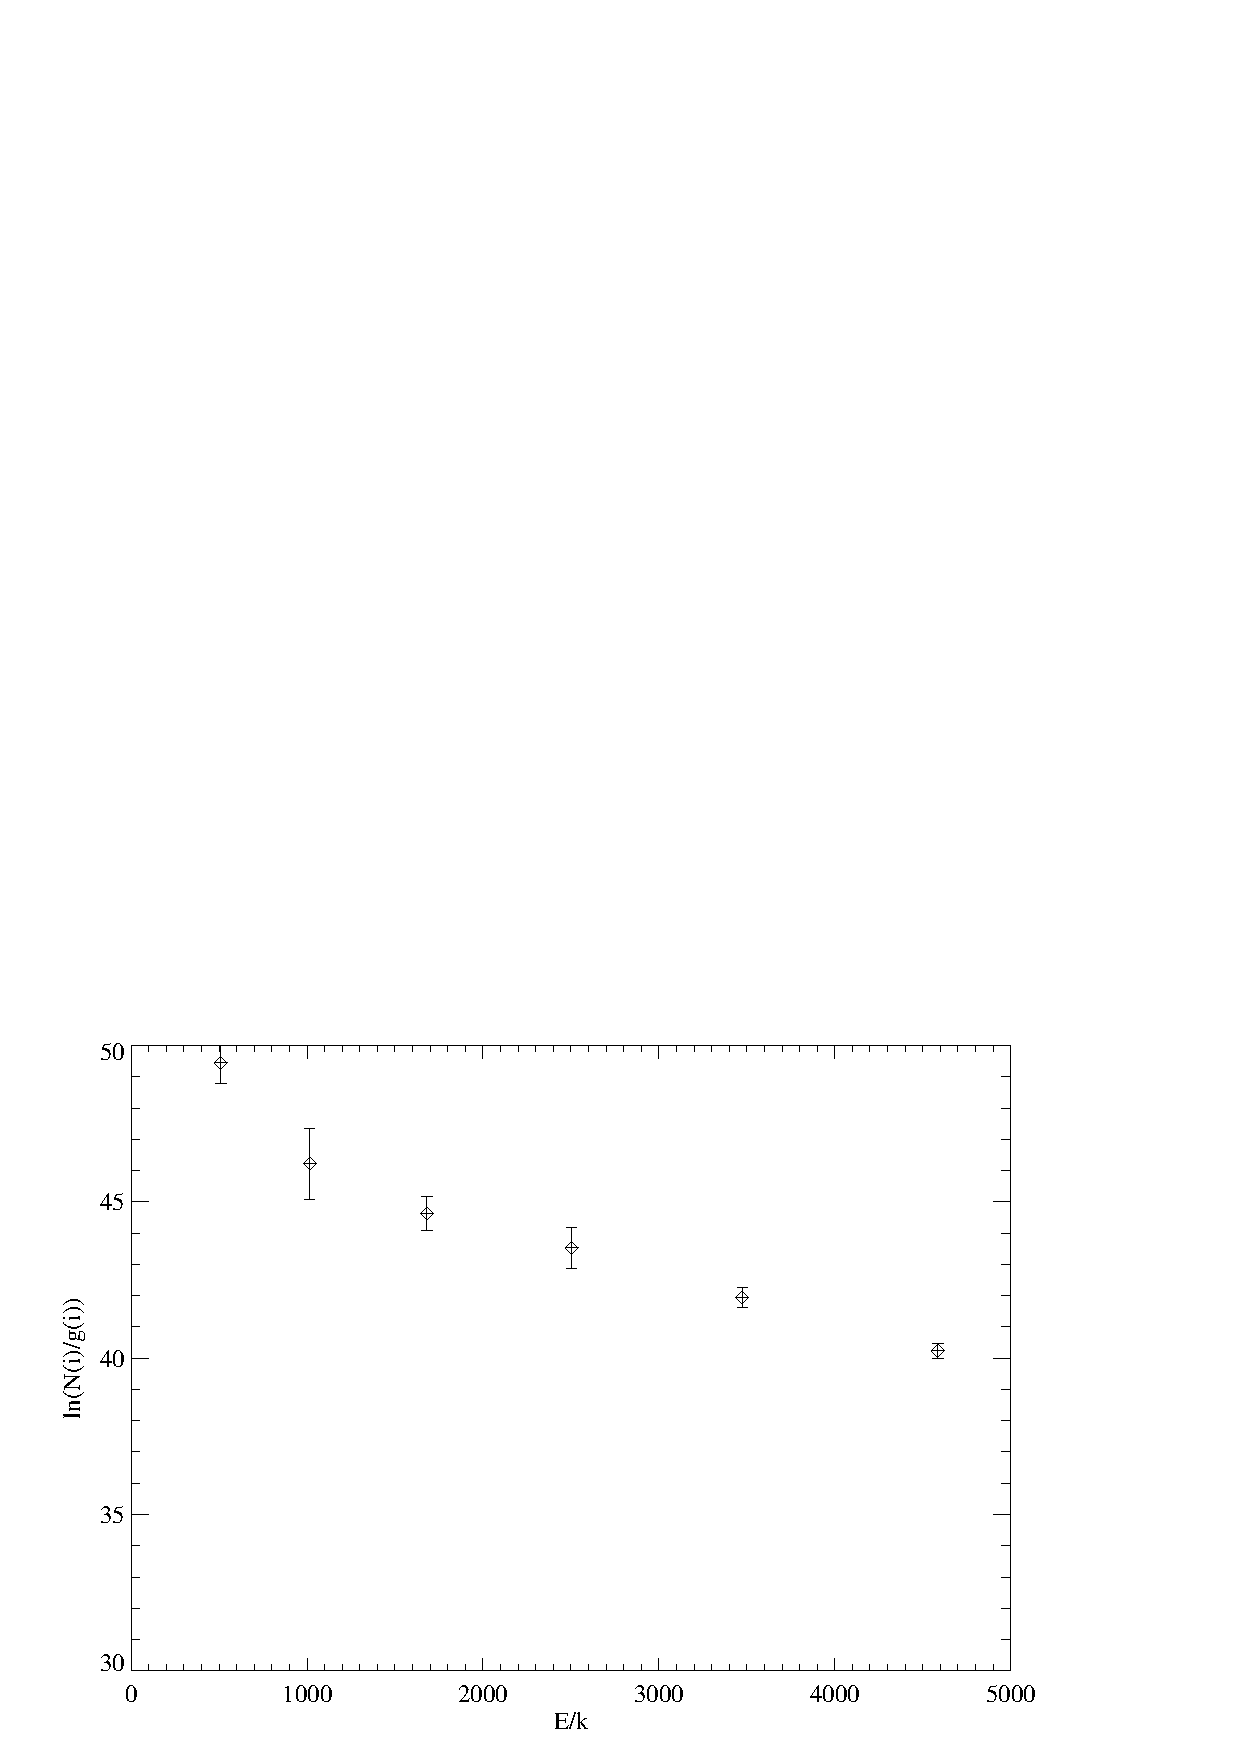
\includegraphics[width=8cm,angle=0]{region2.jpg}}}
\caption{Sample excitation diagrams taken from different regions along the NGC 5194 strip.  The top two excitation diagrams are taken from the different spiral arms at 25 $\mathrm{arcsec^2}$ regions at (RA, Dec) of (202.45, 47.21) and (202.49, 47.18), respectively. The excitation diagram at the bottom is taken from from a 25 $\mathrm{arcsec^2}$ region in the center of \objectname{NGC 5194} at (RA, Dec) of (202.47, 47.19).
\label{fig2}}
\end{figure}



\clearpage
\begin{figure}[!h]
\centerline{\hbox{\hspace{0.0in}
\includegraphics[width=8cm,angle=0]{bw_cold_h2.jpg}}}
\caption{The warm (T = 175 - 275 K) $\mathrm{H_2}$ mass compared to the warm $\mathrm{H_2}$ excitation-temperature distribution.  The warm $\mathrm{H_2}$ excitation-temperature and mass distributions are derived from the fit to the excitation diagrams across the strip for the $\mathrm{H_2}$ S(0), $\mathrm{H_2}$ S(1), and $\mathrm{H_2}$ S(2) lines.  Mass density contour levels are 0.45, 0.28, 0.23, 0.17, 0.11, and 0.06 $\mathrm{M_\sun}$/$\mathrm{pc^2}$). Contours represent the mass within a 5.5 x 10^{4} $\mathrm{pc^2}$ area. The grey-scale represents the excitation-temperature distribution (in units of Kelvin).  The non-rectangular shape to the map is due to the slight offset of the Spitzer IRS SL strip relative to the LL strip.  \label{fig3}}
\end{figure}

\clearpage
\begin{figure}[!h]
\centerline{\hbox{\hspace{0.0in}
\includegraphics[width=8cm,angle=0]{bw_warm_h2.jpg}}}
\caption{The hot (T = 500 - 1000 K) $\mathrm{H_2}$ mass compared to the hot $\mathrm{H_2}$ ecitation-temperature distribution.  The hot $\mathrm{H_2}$ excitation-temperature and mass distributions are derived from the fit to the ecitation diagrams across the strip for the $\mathrm{H_2}$ S(2), $\mathrm{H_2}$ S(3), $\mathrm{H_2}$ S(4), and $\mathrm{H_2}$ S(5) lines.  Mass density contour levels are at 10\% of the maximum mass density (0.002 $\mathrm{M_\sun}$/$\mathrm{pc^2}$). Contours represent the amount of mass of the hot $\mathrm{H_2}$ within a 5.5 x 10^{4} $\mathrm{pc^2}$ area.  The grey-scale represents the excitation-temperature distribution (in units of Kelvin).  Note that the due to lack of $\mathrm{H_2}$ detection from the higher J lines a greater distances from the nucleus of NGC 5194, we are unable to map the hot $\mathrm{H_2}$ distributions across the entire strip as we have done for the warm $\mathrm{H_2}$ distribution.\label{fig4}}
\end{figure}

\clearpage
\begin{figure}[!h]
\centerline{\hbox{\hspace{0.0in}
\includegraphics[width=8cm,angle=0]{bw_h2_mass_compare.jpg}}}
\caption{The warm (175K - 275 K) $\mathrm{H_2}$ mass (in grey-scale) compared to the hot (T = 500 - 1000 K) $\mathrm{H_2}$ mass (in contours).  Contours levels for the hot $\mathrm{H_2}$ mass distribution are at 10\% of the maximum mass density (0.002 $\mathrm{M_\sun}$/$\mathrm{pc^2}$). Contours represent the amount of mass of the hot $\mathrm{H_2}$ within a 5.5 x ${10^{4}}$ $\mathrm{pc^2}$ area.  The grey-scale is in units of $\mathrm{M_\sun}$/$\mathrm{pc^2}$ and also represents the amount of mass of the warm $\mathrm{H_2}$ within a 5.5 x ${10^{4}}$ $\mathrm{pc^2}$ area. \label{fig5}}
\end{figure}


\clearpage

\begin{figure}[!h]
\centerline{\hbox{ \hspace{0.0in} 
\includegraphics[width=8cm,angle=0]{bw_co_h2s0.jpg}
\hspace{0.1in}
\includegraphics[width=8cm,angle=0]{bw_co_h2s1.jpg}}}
\end{figure}

\begin{figure}[!h]
\centerline{\hbox{\hspace{0.0in}
\includegraphics[width=8cm,angle=0]{bw_co_h2s2.jpg}
\hspace{0.1in}
\includegraphics[width=8cm,angle=0]{bw_co_h2s3.jpg}}}
\caption{Comparison of the CO emission to the $\mathrm{H_2}$ S(0) (top left),  $\mathrm{H_2}$ S(1) (top right),  $\mathrm{H_2}$ S(2) (bottom left),  and $\mathrm{H_2}$ S(3) (bottom right) emission.  The CO emission maps are in units of Jy beam $\mathrm{s^{-1}}$.  Contour levels for $\mathrm{H_2}$ S(0), $\mathrm{H_2}$ S(1), $\mathrm{H_2}$ S(2), and $\mathrm{H_2}$ S(3) are at the same levels as those used in Figure 1 and Figure 2.\label{fig6}}
\end{figure}

\clearpage

\begin{figure}[!h]
\centerline{\hbox{\hspace{0.0in}
\includegraphics[width=8cm,angle=0]{co_v_warm_h2.jpg}}}
\caption{Comparison of the cold $\mathrm{H_2}$ (as traced by the CO emission) to the warm (T = 150-275 K) $\mathrm{H_2}$ mass.  Cold $\mathrm{H_2}$ mass is in units of $\mathrm{M_\sun}$. Warm $\mathrm{H_2}$ mass contours are the same as in Figure 4.\label{fig7}}
\end{figure}

\clearpage

\begin{figure}[!h]
\centerline{\hbox{\hspace{0.0in}
\includegraphics[width=8cm,angle=0]{co_v_hot_h2.jpg}}}
\caption{Comparison of the cold $\mathrm{H_2}$ (as traced by CO emission) to the hot (T = 500-1000 K) $\mathrm{H_2}$ mass.  Cold $\mathrm{H_2}$ mass is in units of $\mathrm{M_\sun}$. Hot $\mathrm{H_2}$ mass contours are the same as in Figure 5.\label{fig8}}
\end{figure}

\begin{figure}[!h]
\centerline{\hbox{ \hspace{0.0in} 
\includegraphics[width=8cm,angle=0]{oiv_v_warm_paper.jpg}
\hspace{0.1in}
\includegraphics[width=8cm,angle=0]{oiv_v_hot_paper.jpg}}}
\caption{$Left$:  Comparison of the [OIV](25.89 \micron) emission (in grey) to the warm (T = 175 K - 275 K) $\mathrm{H_2}$ mass distribution (in contours).  Hot $\mathrm{H_2}$ mass contours are the same as in Figure 4.  $Right$: Comparison of the [OIV](25.89 \micron) emission (in grey) to the hot (T = 500 - 1000 K) $\mathrm{H_2}$ mass distribution (in contours).  Hot $\mathrm{H_2}$ mass contours are the same as in Figure 5.  The [OIV](25.89 \micron) emission is in units of W/$\mathrm{m^2}$.\label{fig9}}
\end{figure}

\clearpage

\begin{figure}[!t]
\centerline{\hbox{ \hspace{0.0in} 
\includegraphics[width=8cm,angle=0]{bw_x_v_cold_h2.jpg}
\hspace{0.1in}
\includegraphics[width=8cm,angle=0]{bw_x_v_warm_h2.jpg}}}
\caption{$Left$:  Comparison of the 0.5 - 10 keV x-ray emission band (in grey) to the warm (T = 175 - 275 K) $\mathrm{H_2}$ mass distribution (in contours).  X-ray emission is in units of counts.  $\mathrm{H_2}$ mass contours are the same as in Figure 4.  $Right$: Comparison of the 0.5 - 10 keV x-ray emission band (in grey) to the hot (T = 500 - 1000 K) $\mathrm{H_2}$ mass distribution (in contours).  The $\mathrm{H_2}$ mass distribution contours are the same as in Figure 5.\label{fig10}}
\end{figure}

\clearpage

\begin{figure}[!h]
\centerline{\hbox{ \hspace{0.0in} 
\includegraphics[width=8cm,angle=0]{bw_x_v_h2s2.jpg}
\hspace{0.1in}
\includegraphics[width=8cm,angle=0]{bw_x_v_h2s3.jpg}}}
\end{figure}

\begin{figure}[!h]
\centerline{\hbox{\hspace{0.0in}
\includegraphics[width=8cm,angle=0]{bw_x_v_h2s4.jpg}
\hspace{0.1in}
\includegraphics[width=8cm,angle=0]{bw_x_v_h2s5.jpg}}}
\caption{Comparison of 0.5 - 10 keV x-ray emission band (in grey) to the $\mathrm{H_2}$ S(2) (top left), $\mathrm{H_2}$ S(3) (top right), $\mathrm{H_2}$ S(4) (bottom left), and $\mathrm{H_2}$ S(5) (bottom right) emission in the nuclear region of NGC 5194.  X-ray emission is in units of counts.  The $\mathrm{H_2}$ S(2) and $\mathrm{H_2}$ S(3) emission contours are at 10\% of their peak values (2.20 x ${10^{-18}}$ and 1.35 x ${10^{-17}}$ W/$\mathrm{m^2}$, respectively).  The $\mathrm{H_2}$ S(4) contours are at  2.0 x ${10^{-18}}$and 1.0 x ${10^{-18}}$ W/$\mathrm{m^2}$ and the $\mathrm{H_2}$ S(5) contours are at 7.3 x ${10^{-18}}$, 4.0 x ${10^{-18}}$, and 8.0 x ${10^{-19}}$ W/$\mathrm{m^2}$.\label{fig11}}
\end{figure}



\clearpage


\begin{deluxetable}{cccccc}
\tabletypesize{\scriptsize}
\rotate
\tablecaption{$\mathrm{H_2}$ Parameters\label{tbl-1}}
\tablewidth{0pt}
\tablehead{
\colhead{Transition} & \colhead{Wavelength (\micron)} & \colhead{Rotational State (J)} & \colhead{Energy (E/k)} & \colhead{A ($\mathrm{s^{-1}})} & \colhead{Statistical Weight (g)} 
}
\startdata
$\mathrm{H_2}$(0-0)S(0) & 28.22 & 2 & 510 & 2.94x${10^{-11}}$ & 5 \\
$\mathrm{H_2}$(0-0)S(1) & 17.04 & 3 & 1015 & 4.76x${10^{-10}}$ & 21 \\
$\mathrm{H_2}$(0-0)S(2) & 12.28 & 4 & 1682 & 2.76x${10^{-9}}$ & 9 \\
$\mathrm{H_2}$(0-0)S(3) & 9.66 & 5 & 2504 & 9.84x${10^{-9}}$ & 33 \\
$\mathrm{H_2}$(0-0)S(4) & 8.03 & 6 & 3474 & 2.64x${10^{-8}}$ & 13 \\
$\mathrm{H_2}$(0-0)S(5) & 6.91 & 7 & 4586 & 5.88x${10^{-8}}$ & 45 \\
$\mathrm{H_2}$(0-0)S(6) & 6.11 & 8 & 5829 & 1.14x${10^{-7}}$ & 17 \\
$\mathrm{H_2}$(0-0)S(7) & 5.51 & 9 & 7197 & 2.00x${10^{-7}}$ & 57 \\
\enddata
\tablecomments{The statistical weight (g) is (2$J$ +1)(2$I$+1) where $I$ equals 1 for odd J transitions (ortho transitions) and $I$ equals 0 for even J transitions (para transitions).} 
\end{deluxetable}

\clearpage

\begin{deluxetable}{cccccc}
\tabletypesize{\scriptsize}
\rotate
\tablecaption{Resolution of the $\mathrm{H_2}$ Maps\label{tbl-2}}
\tablewidth{0pt}
\tablehead{
\colhead{Transition} & \colhead{Wavelength (\micron)} & \colhead{Spatial Resolution} & \colhead{\lambda/\delta\lambda}
}
\startdata
$\mathrm{H_2}$(0-0)S(0) & 28.22 & 10".2 & 155  \\
$\mathrm{H_2}$(0-0)S(1) & 17.04 & 6".17 & 185 \\
$\mathrm{H_2}$(0-0)S(2) & 12.28 & 4".37 & 198 \\
$\mathrm{H_2}$(0-0)S(3) & 9.66 & 3".44 & 156 \\
$\mathrm{H_2}$(0-0)S(4) & 8.03 & 2".85 & 129 \\
$\mathrm{H_2}$(0-0)S(5) & 6.91 & 2".46 & 223 \\
\enddata
%\tablecomments{Table lists the resolution of the $\mathrm{H_2}$ lines for which the extinction corrected flux has been mapped across the strip over \objectname{NGC 5194}.} 
\end{deluxetable}




\end{document}

